% Generated by Sphinx.
\def\sphinxdocclass{report}
\documentclass[letterpaper,10pt,spanish]{sphinxmanual}
\usepackage[utf8]{inputenc}
\DeclareUnicodeCharacter{00A0}{\nobreakspace}
\usepackage{cmap}
\usepackage[T1]{fontenc}
\usepackage{babel}
\usepackage{times}
\usepackage[Sonny]{fncychap}
\usepackage{longtable}
\usepackage{sphinx}
\usepackage{multirow}

\addto\captionsspanish{\renewcommand{\figurename}{Figura }}
\addto\captionsspanish{\renewcommand{\tablename}{Tabla }}
\floatname{literal-block}{Lista }



\title{Scanner Vial Documentation}
\date{30 de July de 2015}
\release{1.0}
\author{Almonacid, Huincalef, Ingravallo, Martinez, Navarro, Urrutia, van Haaster}
\newcommand{\sphinxlogo}{}
\renewcommand{\releasename}{Publicación}
\makeindex

\makeatletter
\def\PYG@reset{\let\PYG@it=\relax \let\PYG@bf=\relax%
    \let\PYG@ul=\relax \let\PYG@tc=\relax%
    \let\PYG@bc=\relax \let\PYG@ff=\relax}
\def\PYG@tok#1{\csname PYG@tok@#1\endcsname}
\def\PYG@toks#1+{\ifx\relax#1\empty\else%
    \PYG@tok{#1}\expandafter\PYG@toks\fi}
\def\PYG@do#1{\PYG@bc{\PYG@tc{\PYG@ul{%
    \PYG@it{\PYG@bf{\PYG@ff{#1}}}}}}}
\def\PYG#1#2{\PYG@reset\PYG@toks#1+\relax+\PYG@do{#2}}

\expandafter\def\csname PYG@tok@w\endcsname{\def\PYG@tc##1{\textcolor[rgb]{0.73,0.73,0.73}{##1}}}
\expandafter\def\csname PYG@tok@nl\endcsname{\let\PYG@bf=\textbf\def\PYG@tc##1{\textcolor[rgb]{0.00,0.13,0.44}{##1}}}
\expandafter\def\csname PYG@tok@gi\endcsname{\def\PYG@tc##1{\textcolor[rgb]{0.00,0.63,0.00}{##1}}}
\expandafter\def\csname PYG@tok@sb\endcsname{\def\PYG@tc##1{\textcolor[rgb]{0.25,0.44,0.63}{##1}}}
\expandafter\def\csname PYG@tok@kr\endcsname{\let\PYG@bf=\textbf\def\PYG@tc##1{\textcolor[rgb]{0.00,0.44,0.13}{##1}}}
\expandafter\def\csname PYG@tok@ne\endcsname{\def\PYG@tc##1{\textcolor[rgb]{0.00,0.44,0.13}{##1}}}
\expandafter\def\csname PYG@tok@gu\endcsname{\let\PYG@bf=\textbf\def\PYG@tc##1{\textcolor[rgb]{0.50,0.00,0.50}{##1}}}
\expandafter\def\csname PYG@tok@o\endcsname{\def\PYG@tc##1{\textcolor[rgb]{0.40,0.40,0.40}{##1}}}
\expandafter\def\csname PYG@tok@vc\endcsname{\def\PYG@tc##1{\textcolor[rgb]{0.73,0.38,0.84}{##1}}}
\expandafter\def\csname PYG@tok@vi\endcsname{\def\PYG@tc##1{\textcolor[rgb]{0.73,0.38,0.84}{##1}}}
\expandafter\def\csname PYG@tok@no\endcsname{\def\PYG@tc##1{\textcolor[rgb]{0.38,0.68,0.84}{##1}}}
\expandafter\def\csname PYG@tok@gp\endcsname{\let\PYG@bf=\textbf\def\PYG@tc##1{\textcolor[rgb]{0.78,0.36,0.04}{##1}}}
\expandafter\def\csname PYG@tok@sx\endcsname{\def\PYG@tc##1{\textcolor[rgb]{0.78,0.36,0.04}{##1}}}
\expandafter\def\csname PYG@tok@kn\endcsname{\let\PYG@bf=\textbf\def\PYG@tc##1{\textcolor[rgb]{0.00,0.44,0.13}{##1}}}
\expandafter\def\csname PYG@tok@nb\endcsname{\def\PYG@tc##1{\textcolor[rgb]{0.00,0.44,0.13}{##1}}}
\expandafter\def\csname PYG@tok@nt\endcsname{\let\PYG@bf=\textbf\def\PYG@tc##1{\textcolor[rgb]{0.02,0.16,0.45}{##1}}}
\expandafter\def\csname PYG@tok@k\endcsname{\let\PYG@bf=\textbf\def\PYG@tc##1{\textcolor[rgb]{0.00,0.44,0.13}{##1}}}
\expandafter\def\csname PYG@tok@na\endcsname{\def\PYG@tc##1{\textcolor[rgb]{0.25,0.44,0.63}{##1}}}
\expandafter\def\csname PYG@tok@sd\endcsname{\let\PYG@it=\textit\def\PYG@tc##1{\textcolor[rgb]{0.25,0.44,0.63}{##1}}}
\expandafter\def\csname PYG@tok@vg\endcsname{\def\PYG@tc##1{\textcolor[rgb]{0.73,0.38,0.84}{##1}}}
\expandafter\def\csname PYG@tok@gs\endcsname{\let\PYG@bf=\textbf}
\expandafter\def\csname PYG@tok@cs\endcsname{\def\PYG@tc##1{\textcolor[rgb]{0.25,0.50,0.56}{##1}}\def\PYG@bc##1{\setlength{\fboxsep}{0pt}\colorbox[rgb]{1.00,0.94,0.94}{\strut ##1}}}
\expandafter\def\csname PYG@tok@cp\endcsname{\def\PYG@tc##1{\textcolor[rgb]{0.00,0.44,0.13}{##1}}}
\expandafter\def\csname PYG@tok@se\endcsname{\let\PYG@bf=\textbf\def\PYG@tc##1{\textcolor[rgb]{0.25,0.44,0.63}{##1}}}
\expandafter\def\csname PYG@tok@ge\endcsname{\let\PYG@it=\textit}
\expandafter\def\csname PYG@tok@sh\endcsname{\def\PYG@tc##1{\textcolor[rgb]{0.25,0.44,0.63}{##1}}}
\expandafter\def\csname PYG@tok@kt\endcsname{\def\PYG@tc##1{\textcolor[rgb]{0.56,0.13,0.00}{##1}}}
\expandafter\def\csname PYG@tok@ss\endcsname{\def\PYG@tc##1{\textcolor[rgb]{0.32,0.47,0.09}{##1}}}
\expandafter\def\csname PYG@tok@mi\endcsname{\def\PYG@tc##1{\textcolor[rgb]{0.13,0.50,0.31}{##1}}}
\expandafter\def\csname PYG@tok@err\endcsname{\def\PYG@bc##1{\setlength{\fboxsep}{0pt}\fcolorbox[rgb]{1.00,0.00,0.00}{1,1,1}{\strut ##1}}}
\expandafter\def\csname PYG@tok@gr\endcsname{\def\PYG@tc##1{\textcolor[rgb]{1.00,0.00,0.00}{##1}}}
\expandafter\def\csname PYG@tok@s2\endcsname{\def\PYG@tc##1{\textcolor[rgb]{0.25,0.44,0.63}{##1}}}
\expandafter\def\csname PYG@tok@nd\endcsname{\let\PYG@bf=\textbf\def\PYG@tc##1{\textcolor[rgb]{0.33,0.33,0.33}{##1}}}
\expandafter\def\csname PYG@tok@nc\endcsname{\let\PYG@bf=\textbf\def\PYG@tc##1{\textcolor[rgb]{0.05,0.52,0.71}{##1}}}
\expandafter\def\csname PYG@tok@mh\endcsname{\def\PYG@tc##1{\textcolor[rgb]{0.13,0.50,0.31}{##1}}}
\expandafter\def\csname PYG@tok@gt\endcsname{\def\PYG@tc##1{\textcolor[rgb]{0.00,0.27,0.87}{##1}}}
\expandafter\def\csname PYG@tok@mb\endcsname{\def\PYG@tc##1{\textcolor[rgb]{0.13,0.50,0.31}{##1}}}
\expandafter\def\csname PYG@tok@cm\endcsname{\let\PYG@it=\textit\def\PYG@tc##1{\textcolor[rgb]{0.25,0.50,0.56}{##1}}}
\expandafter\def\csname PYG@tok@kd\endcsname{\let\PYG@bf=\textbf\def\PYG@tc##1{\textcolor[rgb]{0.00,0.44,0.13}{##1}}}
\expandafter\def\csname PYG@tok@gh\endcsname{\let\PYG@bf=\textbf\def\PYG@tc##1{\textcolor[rgb]{0.00,0.00,0.50}{##1}}}
\expandafter\def\csname PYG@tok@go\endcsname{\def\PYG@tc##1{\textcolor[rgb]{0.20,0.20,0.20}{##1}}}
\expandafter\def\csname PYG@tok@bp\endcsname{\def\PYG@tc##1{\textcolor[rgb]{0.00,0.44,0.13}{##1}}}
\expandafter\def\csname PYG@tok@il\endcsname{\def\PYG@tc##1{\textcolor[rgb]{0.13,0.50,0.31}{##1}}}
\expandafter\def\csname PYG@tok@si\endcsname{\let\PYG@it=\textit\def\PYG@tc##1{\textcolor[rgb]{0.44,0.63,0.82}{##1}}}
\expandafter\def\csname PYG@tok@mf\endcsname{\def\PYG@tc##1{\textcolor[rgb]{0.13,0.50,0.31}{##1}}}
\expandafter\def\csname PYG@tok@nn\endcsname{\let\PYG@bf=\textbf\def\PYG@tc##1{\textcolor[rgb]{0.05,0.52,0.71}{##1}}}
\expandafter\def\csname PYG@tok@sr\endcsname{\def\PYG@tc##1{\textcolor[rgb]{0.14,0.33,0.53}{##1}}}
\expandafter\def\csname PYG@tok@sc\endcsname{\def\PYG@tc##1{\textcolor[rgb]{0.25,0.44,0.63}{##1}}}
\expandafter\def\csname PYG@tok@kc\endcsname{\let\PYG@bf=\textbf\def\PYG@tc##1{\textcolor[rgb]{0.00,0.44,0.13}{##1}}}
\expandafter\def\csname PYG@tok@s1\endcsname{\def\PYG@tc##1{\textcolor[rgb]{0.25,0.44,0.63}{##1}}}
\expandafter\def\csname PYG@tok@ow\endcsname{\let\PYG@bf=\textbf\def\PYG@tc##1{\textcolor[rgb]{0.00,0.44,0.13}{##1}}}
\expandafter\def\csname PYG@tok@kp\endcsname{\def\PYG@tc##1{\textcolor[rgb]{0.00,0.44,0.13}{##1}}}
\expandafter\def\csname PYG@tok@gd\endcsname{\def\PYG@tc##1{\textcolor[rgb]{0.63,0.00,0.00}{##1}}}
\expandafter\def\csname PYG@tok@c1\endcsname{\let\PYG@it=\textit\def\PYG@tc##1{\textcolor[rgb]{0.25,0.50,0.56}{##1}}}
\expandafter\def\csname PYG@tok@s\endcsname{\def\PYG@tc##1{\textcolor[rgb]{0.25,0.44,0.63}{##1}}}
\expandafter\def\csname PYG@tok@nf\endcsname{\def\PYG@tc##1{\textcolor[rgb]{0.02,0.16,0.49}{##1}}}
\expandafter\def\csname PYG@tok@nv\endcsname{\def\PYG@tc##1{\textcolor[rgb]{0.73,0.38,0.84}{##1}}}
\expandafter\def\csname PYG@tok@mo\endcsname{\def\PYG@tc##1{\textcolor[rgb]{0.13,0.50,0.31}{##1}}}
\expandafter\def\csname PYG@tok@m\endcsname{\def\PYG@tc##1{\textcolor[rgb]{0.13,0.50,0.31}{##1}}}
\expandafter\def\csname PYG@tok@ni\endcsname{\let\PYG@bf=\textbf\def\PYG@tc##1{\textcolor[rgb]{0.84,0.33,0.22}{##1}}}
\expandafter\def\csname PYG@tok@c\endcsname{\let\PYG@it=\textit\def\PYG@tc##1{\textcolor[rgb]{0.25,0.50,0.56}{##1}}}

\def\PYGZbs{\char`\\}
\def\PYGZus{\char`\_}
\def\PYGZob{\char`\{}
\def\PYGZcb{\char`\}}
\def\PYGZca{\char`\^}
\def\PYGZam{\char`\&}
\def\PYGZlt{\char`\<}
\def\PYGZgt{\char`\>}
\def\PYGZsh{\char`\#}
\def\PYGZpc{\char`\%}
\def\PYGZdl{\char`\$}
\def\PYGZhy{\char`\-}
\def\PYGZsq{\char`\'}
\def\PYGZdq{\char`\"}
\def\PYGZti{\char`\~}
% for compatibility with earlier versions
\def\PYGZat{@}
\def\PYGZlb{[}
\def\PYGZrb{]}
\makeatother

\renewcommand\PYGZsq{\textquotesingle}

\begin{document}
\shorthandoff{"}
\maketitle
\tableofcontents
\phantomsection\label{index::doc}



\chapter{Patología de los Pavimentos}
\label{index:welcome-to-scanner-vial-s-documentation}\label{index:patologia-de-los-pavimentos}

\section{Introducción}
\label{patologia/introduccion::doc}\label{patologia/introduccion:patologia-introduccion}\label{patologia/introduccion:introduccion}
La evaluación del estado y la condición de una carretera es parte fundamental
en un sistema de gestión de infraestructura vial, para garantizar la
continuidad de ésta en el tiempo, brindando una buena prestación del servicio.
Es por esta razón, que realizar la evalua­ción de una carretera es una necesidad
para poder determinar las posibles deficiencias y las labores de mantenimiento
que ésta requiera.

Los tres tipos de pavimentos existentes son los siguientes:


\subsection{Pavimento Rígido}
\label{patologia/introduccion:pavimento-rigido}
Estructura compuesta por losas de hormigón cuya resistencia a la flexión es
relativamente elevada.


\subsection{Pavimento Flexible}
\label{patologia/introduccion:pavimento-flexible}
Estructura compuesta por capas donde uno de los materiales presentes es el
asfalto permitiendo la deflexión bajo las cargas.


\subsection{Pavimento Articulado}
\label{patologia/introduccion:pavimento-articulado}
Estructura construida con adoquines de concreto o de ladrillo, la transmisión
de cargas es independiente para cada elemento.
Para cada uno de los deterioros se detallan los siguientes cinco aspectos:
\begin{itemize}
\item {} 
Breve descripción.

\item {} 
Clasificación, según características, de los tres niveles de severidad: baja, media y alta.

\item {} 
Procedimiento de medición y cuantificación.

\item {} 
Operaciones de reparación.

\item {} 
Esquemas y/o fotografías explicativas.

\end{itemize}
\begin{figure}[htbp]
\centering

\scalebox{0.800000}{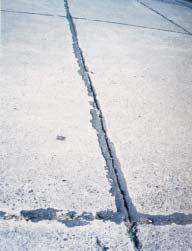
\includegraphics{sellado1.png}}
\end{figure}
\begin{quote}
\end{quote}


\section{Pavimentos Rígidos}
\label{patologia/rigidos::doc}\label{patologia/rigidos:patologia-rigidos}\label{patologia/rigidos:pavimentos-rigidos}

\subsection{Deficiencia de Sellado}
\label{patologia/rigidos:deficiencia-de-sellado}

\subsection{Losas Desniveladas}
\label{patologia/rigidos:losas-desniveladas}

\subsection{Grietas}
\label{patologia/rigidos:grietas}

\subsection{Desintegración}
\label{patologia/rigidos:desintegracion}

\subsection{Baches}
\label{patologia/rigidos:baches}

\subsection{Levantamiento}
\label{patologia/rigidos:levantamiento}

\subsection{Escalonamiento De Juntas O Grietas}
\label{patologia/rigidos:escalonamiento-de-juntas-o-grietas}

\subsection{Descenso De Banquinas}
\label{patologia/rigidos:descenso-de-banquinas}

\subsection{Separación Banquina – Pavimento}
\label{patologia/rigidos:separacion-banquina-pavimento}

\subsection{Parches Deteriorados}
\label{patologia/rigidos:parches-deteriorados}\begin{quote}
\end{quote}


\section{Pavimentos Flexibles}
\label{patologia/flexibles:patologia-flexibles}\label{patologia/flexibles::doc}\label{patologia/flexibles:pavimentos-flexibles}

\subsection{Exudación}
\label{patologia/flexibles:exudacion}

\subsection{Ahuellamiento Y Depresiones}
\label{patologia/flexibles:ahuellamiento-y-depresiones}

\subsection{Grietas}
\label{patologia/flexibles:grietas}

\subsection{Hundimiento Del Borde Y Ahuellamiento}
\label{patologia/flexibles:hundimiento-del-borde-y-ahuellamiento}

\subsection{Baches}
\label{patologia/flexibles:baches}

\subsection{Pérdida Local De Áridos}
\label{patologia/flexibles:perdida-local-de-aridos}

\subsection{Pulimiento o Peladuras}
\label{patologia/flexibles:pulimiento-o-peladuras}

\subsection{Deformación}
\label{patologia/flexibles:deformacion}\begin{quote}
\end{quote}


\section{Pavimentos Articulados}
\label{patologia/articulados::doc}\label{patologia/articulados:pavimentos-articulados}\label{patologia/articulados:patologia-articulados}

\subsection{Abultamiento}
\label{patologia/articulados:abultamiento}

\subsection{Ahuellamiento}
\label{patologia/articulados:ahuellamiento}

\subsection{Depresiones}
\label{patologia/articulados:depresiones}

\subsection{Desgaste Superficial / Pérdida De Arena}
\label{patologia/articulados:desgaste-superficial-perdida-de-arena}

\subsection{Desplazamiento De Bordes y/o Juntas}
\label{patologia/articulados:desplazamiento-de-bordes-y-o-juntas}

\subsection{Fracturamientos}
\label{patologia/articulados:fracturamientos}

\subsection{Escalonamiento Entre Adoquines}
\label{patologia/articulados:escalonamiento-entre-adoquines}

\subsection{Juntas Abiertas}
\label{patologia/articulados:juntas-abiertas}

\subsection{Vegetación En La Calzada}
\label{patologia/articulados:vegetacion-en-la-calzada}

\chapter{Sistema}
\label{index:sistema}\begin{description}
\item[{Problematica del municipio}] \leavevmode
Introducción

\item[{Relevamiento de fallas}] \leavevmode
Reporte de los vecinos (Anonimos)
Seguimiento de los reportes
Seguimiento de los montos
Verificacion del ingeniero y comletamiento de datos

\end{description}

Identidad de las fallas

Visualizacion y seguimiento en redes sociales

Tipificacion de las fallas

Deteccion automatica de fallas

Analisis de fallas


\chapter{Indices and tables}
\label{index::doc}\label{index:indices-and-tables}\begin{itemize}
\item {} 
\DUspan{xref,std,std-ref}{genindex}

\item {} 
\DUspan{xref,std,std-ref}{modindex}

\item {} 
\DUspan{xref,std,std-ref}{search}

\end{itemize}



\renewcommand{\indexname}{Índice}
\printindex
\end{document}
